\section{Visuals}


\begin{frame}{Graphical information}
    \begin{wrapfigure}{r}{0.40\textwidth}
	\centering
    	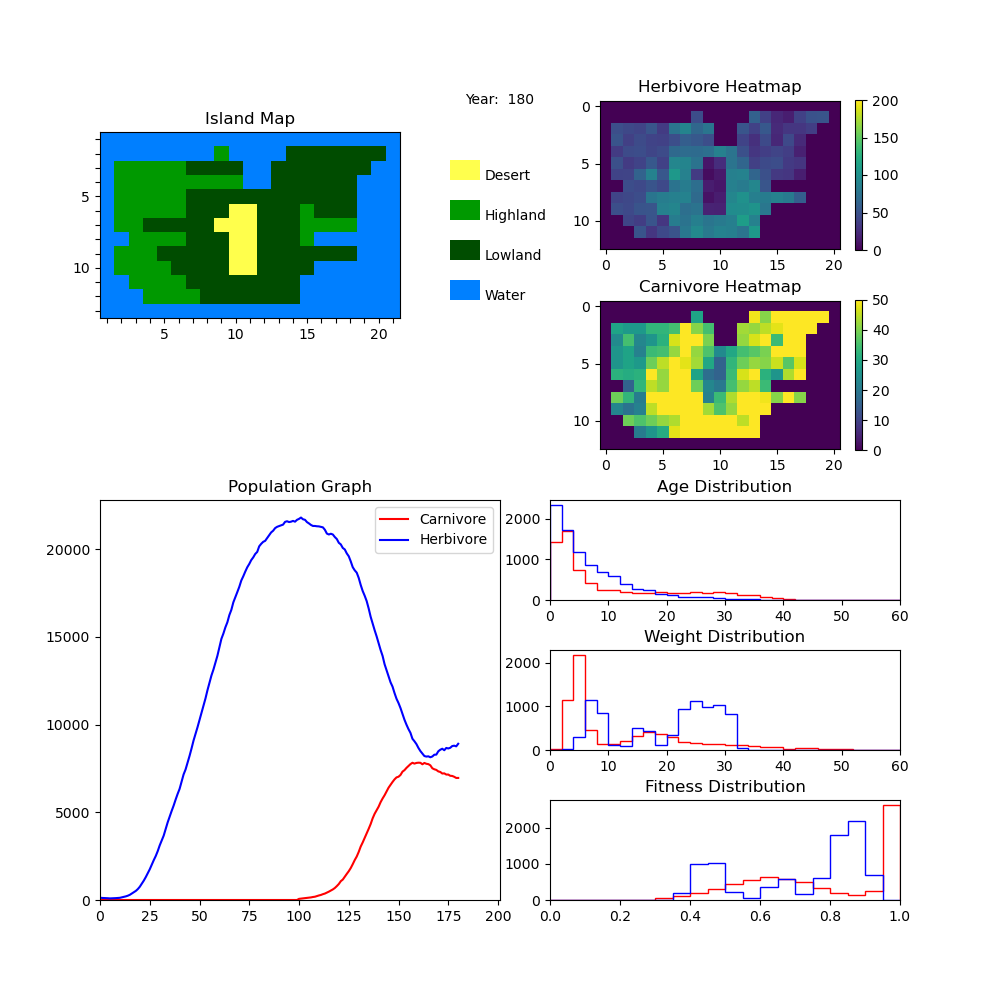
\includegraphics[scale=0.2]{test/test3_00180}
    \end{wrapfigure}
    Display features:
	\pause
    \begin{itemize}[<+->]
        \item Display current year
        \item Display the island geography
        \item Display informational graphs
        \item Ability to save images of the simulation
        \item Ability to set limits and graphical update step
    \end{itemize}
\end{frame}

\begin{frame}{Graphical handling}
    How does the graphics work?

    \pause 	1. The engine stores key information inside itself

    \pause 	2. The interface grabs that information

    \pause 	3. Then graphics takes information from the interface and processes it

\end{frame}
